\documentclass{article}
\usepackage[a4paper, margin=2.5cm]{geometry}
\usepackage{Csharp}
\usepackage[ngerman]{babel}
\lstset{
	basicstyle=\tiny
}

\usepackage{graphicx,capt-of}
\graphicspath{ {images/} }

\newcommand{\q}[1]{\textbf{#1}}
\begin{document}

\title{
{\Huge Aufgabe 4\\Schrebergärten}\\
\vspace{.5cm}
\begin{large}
Team-Name: Bruteforce\\
Team-ID: 00139\\
Bearbeiter:\\ 
\end{large}
\begin{normalsize}
P1,
P3,
P4,
P2
\end{normalsize}
}
\author{}
\date{}
\maketitle
\vspace{5cm}
\tableofcontents
\newpage
\begin{flushleft}
		
\section{Schrebergärten}
\subsection{Lösungsansatz}
In dieser Aufgabe sollen rechteckige Flächen möglichst platzsparend angeordnet werden bzw. so, dass ihre \textit{Bounding Box} eine möglichst geringe Fläche hat. Wir haben uns dazu entschieden einen Evolutionsalgorithmus für diese Problem einzusetzen. Konkret erzeugen wir eine zufällig generierte Menge von Anordnungen von Gärten (1), wählen davon die besten aus (2) und generieren aus ihnen wieder eine neue Menge (3) und springen zu Schritt (2). Dies ahmt den Prozess der natürlichen Evolution nach und generiert über mehrere Iterationen günstige Approximationslösungen für das Problem.  

\subsection{Implementierung}
\label{Implementierung}

Bei dem Evolutionsalgorithmus haben wir uns für eine objektorientierte Modellierung des Prozesses entschieden. Dazu haben wir folgende Klassen implementiert: eine \q{Rect}-Klasse, die ein Rechteck repräsentiert und Daten wie z.B. x,y-Koordinaten, Länge und Breite speichert; eine \q{RectAttempt}-Klasse, die eine mögliche Anordnung von Schrebergärten (dargestellt als eine Liste von Rechtecken) darstellt und eine \q{Evolver}-Klasse, welche Generationen von \q{RectAttempt}-Instanzen erzeugt, die besten über eine Fitness-Funktion auswählt, diese zufällig miteinander kreuzt und mutiert und somit eine Folgegeneration erhält, welche dann die nächste Parentalgeneration bildet. %Unterteilen, TOO LONG SENTENCE -100BE   

\newpage
\subsection{Beispiel}
Geben wir z.B. das Beispiel 3 von der BwInf-Seite ein:\\
\begin{center}
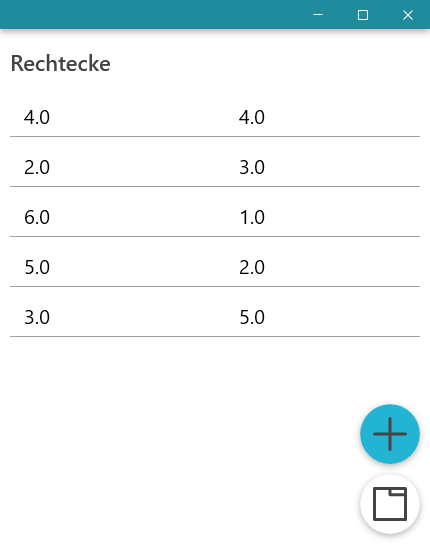
\includegraphics[scale=.5]{schreber3}
\end{center}

und starten das Programm mit folgenden Einstellungen:
\begin{center}
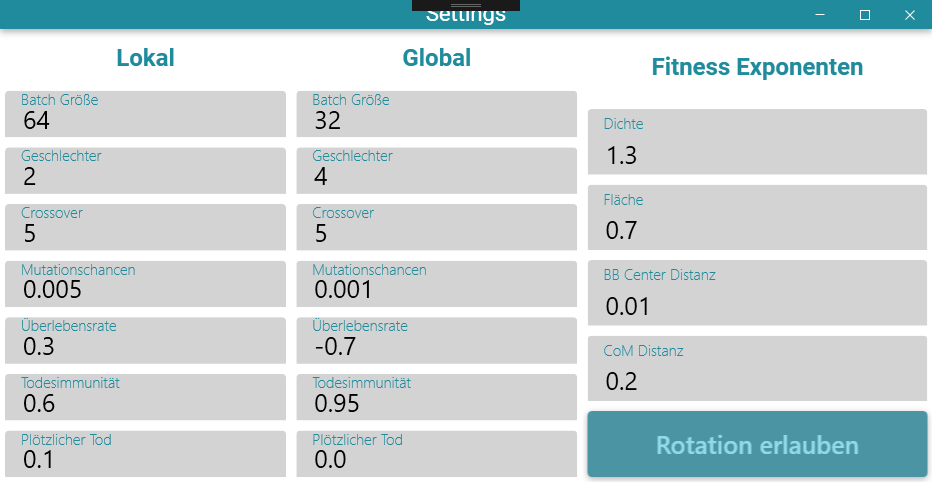
\includegraphics[scale=.5]{schrebersettings}
\end{center}

so erhalten wir nach ca. 2500 Iterationen folgendes Ergebnis: 
\begin{center}
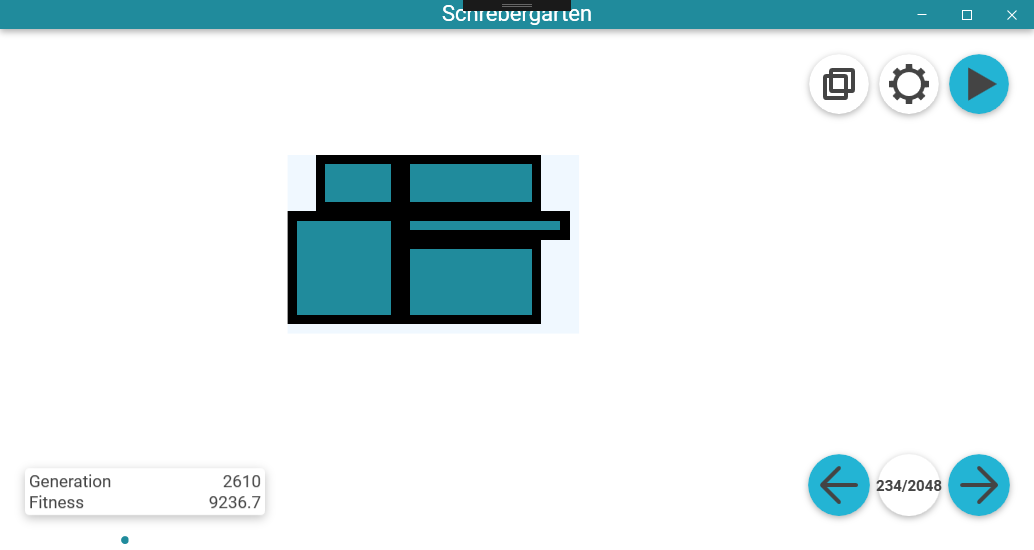
\includegraphics[scale=.5]{schreberresults}
\end{center}

\newpage
\subsection{Code}

\subsubsection{\q{RectAttempt}-Klasse}
\begin{Csharp}
using RectFitness = System.Func<double, double, double, double, double>;

public class RectAttempt : IEvolvable
{
    public List<Rect> rects;

    public double Fitness { get; private set; }
    public RectFitness rectFitness;
    public bool allowRotation;

    public RectAttempt(List<Rect> rects, RectFitness rectFitness, bool allowRotation)
    {
        this.rects = rects;
        this.rectFitness = rectFitness;
        this.allowRotation = allowRotation;
    }
    
    public RectAttempt(RectAttempt toClone) : 
    	this(toClone.rects.Select(x => new Rect(x)).ToList(),
    	toClone.rectFitness,
    	toClone.allowRotation)
    { }

    public Rect BoundingBox()
    {
        if (rects.Count == 0) return new Rect();
        double XStart = rects.Min(x => x.XStart);
        double YStart = rects.Min(x => x.YStart);
        double XEnd   = rects.Max(x => x.XEnd);
        double YEnd   = rects.Max(x => x.YEnd);

        return new Rect((XStart + XEnd) / 2f, (YStart + YEnd) / 2f, XEnd - XStart, YEnd - YStart);
    }

    public void CalculateFitness()
    {
        if (CheckCollisions()) Fitness = -1f;
        else
        {
            Rect boundingBox = BoundingBox();

            double CenterDistance =
                rects.Average(x => Math.Sqrt(
                    Math.Pow(x.XCenter - boundingBox.XCenter, 2) +
                    Math.Pow(x.YCenter - boundingBox.YCenter, 2)
                ));

            Rect averageBox = new Rect(
                rects.Average(x => x.XCenter), rects.Average(x => x.YCenter), 0, 0);

            double WeightedCenterDistance =
                rects.Average(x => 
                    Math.Sqrt(Math.Pow(x.XCenter - averageBox.XCenter, 2)
                    + Math.Pow(x.YCenter - averageBox.YCenter, 2)));

            double Density =
                rects.Average(x => rects.Average(y => 
                    Math.Sqrt(Math.Pow(x.XCenter - y.XCenter, 2)
                    + Math.Pow(x.YCenter - y.YCenter, 2) )));

            Fitness = rectFitness(
            	Density, 
            	boundingBox.Area, 
            	CenterDistance,
            	WeightedCenterDistance);
        }
    }

    // Nimmt an, dass alle RectAttempts im gleichen Format sind (gleiche Menge an Rechtecken etc.)
    public IEvolvable Crossover(IEnumerable<IEvolvable> other, int crossovers, Random random)
    {
        List<RectAttempt> parents = other.Select(x => (RectAttempt)x).Union(new[] { this }).ToList();

        List<int> crossoverSpots = new List<int>(crossovers);
        int geneCount = rects.Count * 2;
        for (int i = 0; i < crossovers; i++)
        {
            int nextSpot;

            while (crossoverSpots.Contains(nextSpot = random.Next(0, geneCount))) ;

            crossoverSpots.Add(nextSpot);
        }
        crossoverSpots.Sort();

        RectAttempt output = new RectAttempt(this);
        int currentParent = 0;
        for (int i = 0; i < geneCount; i++)
        {
            if (crossoverSpots.Count > 0 && i > crossoverSpots[0])
            {
                currentParent = (currentParent + 1) % parents.Count;
                crossoverSpots.RemoveAt(0);
            }

            if (i % 2 == 0)
            {
                output.rects[i / 2].XCenter = 
                	parents[currentParent].rects[i / 2].XCenter;
            }
            else
            {
                output.rects[i / 2].YCenter = 
                	parents[currentParent].rects[i / 2].YCenter;
            }
        }
        return output;
    }

    public void Mutate(double mutatability, Random random)
    {
        rects.ForEach(x =>
        {
            if (random.NextDouble() < mutatability)
            {
                x.XCenter += random.Next(-2, 3);
                x.YCenter += random.Next(-2, 3);
            }

            if (allowRotation && random.NextDouble() < mutatability)
            {
                double buffer = x.Width;
                x.Width = x.Height;
                x.Height = buffer;
            }
        });
    }

    public bool CheckCollisions()
    {
        for (int i = 0; i < rects.Count - 1; i++)
        {
            Rect rectA = rects[i];
            for (int j = i + 1; j < rects.Count; j++)
            {
                Rect rectB = rects[j];

                if (rectA.Overlap(rectB)) return true; 
            }
        }

        return false;
    }

    public bool EqualRects(RectAttempt obj)
    {
        return allowRotation == obj.allowRotation && rects.SequenceEqual(obj.rects);
    }
}
\end{Csharp}

Die wichtigen Funktionen und Eigenschaften an dieser Stelle ist die
\begin{itemize}
\item \q{rects}-Liste, die die gespeicherte Anordnung repräsentiert,
\item \q{Fitness}-Eigenschaft, die die Optimalität der gespeicherten Anordnung zeigt,
\item \q{Mutate}-Methode welche die zufällige Veränderung der in der Liste von Rechtecken erlaubt,
\item \q{Crossover}-Methode, welche die Kreuzung einer oder mehrerer \q{RectAttempt}-\-Instanzen ermöglicht.
\end{itemize} 

\subsubsection{\q{Evolver}-Klasse und \q{IEvolvable}-Interface}
Die \q{Evolver}-Klasse ist generisch definiert, jedoch werden wir sie hier mit $T = RectAttempt$ erklären. Dabei ist zu bemerken das RectAttempt IEvolvable implementiert.
\begin{Csharp}
public interface IEvolvable
{
    IEvolvable Crossover(IEnumerable<IEvolvable> other, 
    	int crossovers, Random random);
    void Mutate(double mutatability, Random random);
	
    void CalculateFitness(); // Optimierung, nur einmal berechnen
    double Fitness { get; }
}

public class Evolver<T>
    where T : IEvolvable
{
    public Random random;
    public List<T> batch;
    public int batchSize;
    public int genders = 2, crossovers = 1;
    public double mutatability = 0.05f, survivalRate = 0f, failureImmunity = 0.1f, suddenDeath = 0.001f;

    public Evolver(List<T> batch, Random random = null)
    {
        this.batch = batch;
        batchSize = Math.Max(batch.Count, batch.Capacity);

        this.random = random ?? new Random();
    }
        
    public void Generation()
    {
        batch.ForEach(evolvable => evolvable.Mutate(mutatability, random));
        batch.ForEach(evolvable => evolvable.CalculateFitness());
            
        double survivalFitness = survivalRate < 0 ? -survivalRate * batch.Min(x => x.Fitness) + (1 + survivalRate) * batch.Average(x => x.Fitness) :
                                                    survivalRate * batch.Max(x => x.Fitness) + (1 - survivalRate) * batch.Average(x => x.Fitness);

        batch = batch
                .Where(x => (x.Fitness > 0                && random.NextDouble() < failureImmunity  
                            || (x.Fitness >= survivalFitness && random.NextDouble() >= suddenDeath)))
                .ToList();

        if (batch.Count < batchSize)
        {
            WeightedListRandom<T> genePool = new WeightedListRandom<T>(batch, random);

            while (batch.Count < batchSize)
            {
                List<IEvolvable> parents = genePool.Next(genders, x => x.Fitness, false).Select(x => (IEvolvable)x).ToList();

                batch.Add((T)parents[0].Crossover(parents.Skip(1), crossovers, random));
            }
        }
    }
}
\end{Csharp}

Hier ist die \q{Generation}-Methode hervorzuheben. Dabei wird zunächst jeder \q{RectAttempt} der vorherigen Generation zufällig mutiert und seine Fitness wird berechnet
\lstset{
firstnumber=30
}
\begin{Csharp}
batch.ForEach(evolvable => evolvable.Mutate(mutatability, random));
batch.ForEach(evolvable => evolvable.CalculateFitness());
\end{Csharp}

Nun werden alle RectAttempts mit zu geringer Fitness entfernt;
\lstset{
firstnumber=33
}
\begin{Csharp}
double survivalFitness = survivalRate < 0 ? -survivalRate * batch.Min(x => x.Fitness) + (1 + survivalRate) * batch.Average(x => x.Fitness) :
                                             survivalRate * batch.Max(x => x.Fitness) + (1 - survivalRate) * batch.Average(x => x.Fitness);

batch = batch
    .Where(x => x.Fitness > 0 				 && random.NextDouble() < failureImmunity
            || (x.Fitness >= survivalFitness && random.NextDouble() >= suddenDeath))
    .ToList();
\end{Csharp}

Danach wird batch wieder auf seine Orginale Größe gebracht, indem $n$ RectAttempts aus den verbleibenden RectAttemps gewählt werden, wobei $n$ der angegebenen Menge an Geschlechtern entspricht. Die Auswahl wird vorgenommen durch einen gewichteten Zufall, wobei das Gewicht jedes Elementes seiner Fitness entspricht.
Diese ausgewählten Elemente sind die Eltern eines neuen RectAttemps, welches durch aufrufen der Crossover-Methode generiert wird.

\end{flushleft}
\end{document}


